% Proposta E (12/11/2026, pedido do autor): a D ainda precisava de legenda. Esta
% segue o molde da figura "Modelo Completo" do PTG
% (ia/rascunhos/figuras_ptg_removidas/fig08-modelo-completo.png), que o autor achava
% intuitiva: cada seta diz o que carrega, e os dois ramos (direção e risco) se
% juntam numa caixa de decisão. Sem losango, sem legenda, sem fórmula, sem LSTM e
% sem indicadores. Mesmo estilo das fig05/fig06. Fora do TG até o autor decidir.
\documentclass[11pt,border=2pt]{standalone}
\usepackage[T1]{fontenc}
\usepackage[utf8]{inputenc}
\usepackage{mathptmx}
\usepackage{tikz}
\usetikzlibrary{arrows.meta,positioning,calc,shapes.geometric}
\tikzset{
  seta/.style={-{Stealth[length=2.2mm]}, semithick},
  caixa/.style={rectangle, draw, semithick, fill=gray!10, rounded corners=2pt,
                align=center, minimum width=46mm, minimum height=10mm, font=\small},
  dado/.style={trapezium, trapezium left angle=75, trapezium right angle=105, draw,
               semithick, fill=white, align=center, minimum height=9mm, font=\small,
               trapezium stretches body},
  rotulo/.style={font=\footnotesize, align=center, fill=white, inner sep=1.5pt},
}
\begin{document}
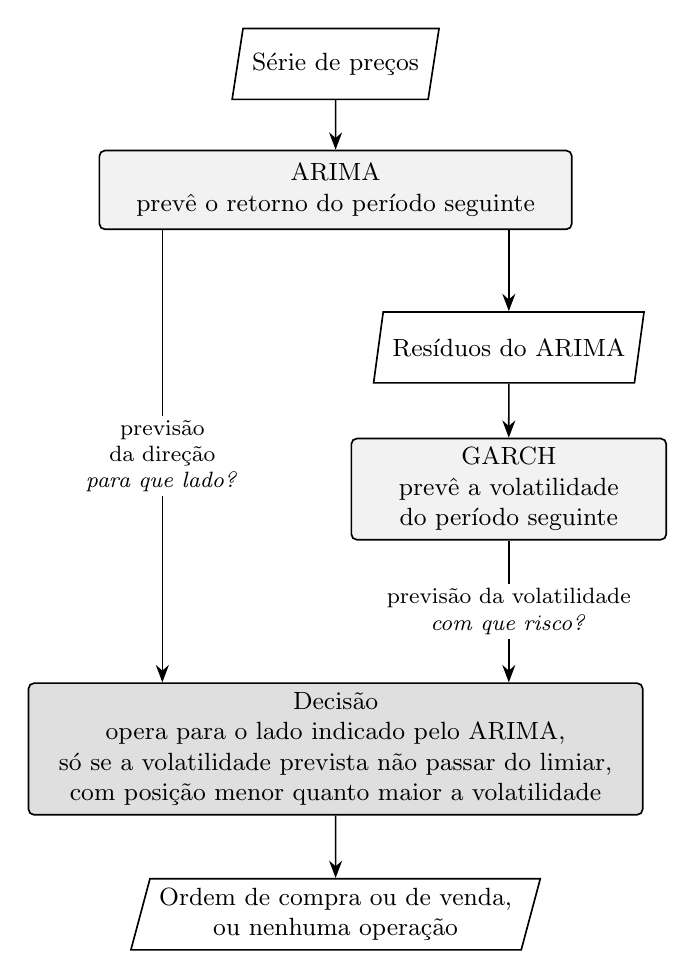
\begin{tikzpicture}
  \node[dado] (ent) at (0,0) {Série de preços};
  \node[caixa, minimum width=60mm] (arima) at (0,-1.6) {ARIMA\\prevê o retorno do período seguinte};
  \node[dado] (res) at (2.2,-3.6) {Resíduos do ARIMA};
  \node[caixa, minimum width=40mm] (garch) at (2.2,-5.4) {GARCH\\prevê a volatilidade\\do período seguinte};
  \node[caixa, fill=gray!25, minimum width=78mm] (dec) at (0,-8.7)
    {Decisão\\opera para o lado indicado pelo ARIMA,\\só se a volatilidade prevista não passar do limiar,\\com posição menor quanto maior a volatilidade};
  \node[dado] (ord) at (0,-10.8) {Ordem de compra ou de venda,\\ou nenhuma operação};

  \draw[seta] (ent) -- (arima);
  \draw[seta] (arima.south -| res.north) -- (res.north);
  \draw[seta] (res) -- (garch);
  \draw[seta] (arima.south -| -2.2,0) -- node[rotulo]{previsão\\da direção\\\textit{para que lado?}} (dec.north -| -2.2,0);
  \draw[seta] (garch) -- node[rotulo]{previsão da volatilidade\\\textit{com que risco?}} (dec.north -| garch);
  \draw[seta] (dec) -- (ord);
\end{tikzpicture}
\end{document}
